\chapter{Sviluppo del progetto}
In questo capitolo verrà descritto lo scopo di questo progetto, i requisiti necessari al suo raggiungimento e i dettagli della sua struttura interna che ne permette il funzionamento. In particolare andremo ad analizzare il class-diagram che mostra le relazioni tra le classi che lo costituiscono e discuteremo delle scelte implementative fatte.

\section{Obiettivo e requisiti}
L'obiettivo di questa tesi è creare un programma in linguaggio Java che sia in grado di ricevere in ingresso la struttura del modello descritta in linguaggio XML e di scrivere in modo automatico il codice NetLogo che possa eseguire la simulazione di interesse, rendendo, quindi, trasparente il processo di scrittura del codice.\\
La scelta del linguaggio XML è dettata dalla sua diffusione, con lo scopo di ridurre le conoscenze preliminari necessarie per l'utilizzo di questo strumento.\\
Per l'analisi del documento XML abbiamo scelto la libreria JDOM2\footnote{http://www.jdom.org/} non inclusa in Java. Il Wold Wide Web Consortium, infatti, ha stabilito uno standard cross-platform e language-indipendent detto DOM (Document Object Model) per la rappresentazione di documenti strutturati (quindi XML, HTML, XHTML) come modello orientato agli oggetti. Il formato JDOM usato dalla libreria è una variazione dello standard disegnata appositamente per Java.\\
Per quanto riguarda la parte della scrittura del codice NetLogo, si ha che gran parte del codice che modella la simulazione rimane fissa al variare dei modelli descritti negli XML, quindi abbiamo pensato di mantenere questa in un semplice file di testo che viene letto e integrato con le informazioni contenute negli oggetti Java. Per le operazioni di lettura e scrittura su file abbiamo usato le classi BufferedReader e PrintWriter che permettono lettura e scrittura di intere linee di testo.\\ 
Lo strumento segue il seguente workflow:
\begin{itemize}
\item analisi del documento XML e costruzione di una rappresentazione della struttura orientata agli oggetti in JDOM attraverso l'omonima libreria
\item costruzione degli oggetti Java per la rappresentazione della simulazione descritta nel modello JDOM 
\item visita degli oggetti Java e scrittura su file del codice NetLogo che eseguirà la simulazione
\end{itemize}

\section{Documento XML}
La struttura del documento XML prevista per il funzionamento del nostro strumento si attiene il più possibile allo standard di formato GraphML\footnote{http://graphml.graphdrawing.org/} (approvato dal W3C) in modo da evitare inconsistenze e incomprensioni, soprattutto per la parte in cui è descritta la topologia dell'ambiente, per la quale questo formato è pienamente adatto.\\
Il file XML è suddiviso in tre sezioni distinte:
\begin{itemize}
\item \texttt{Graph}
\item \texttt{Behaviors}
\item \texttt{System}
\end{itemize} 
\texttt{Graph} rappresenta la topologia dell'ambiente in cui gli attori si muovono, ed è descritta sotto-forma di grafo con \texttt{edges} che rappresentano le strade e \texttt{nodes} che rappresentano gli incroci. Gli edges possono essere \texttt{directed} e \texttt{undirected}, per ognuno di essi vengono specificati peso e larghezza. I nodes invece possono essere di tre tipi: normal, entry o exit. Per tutti e tre i tipi vengono specificate coordinate spaziali e dimensioni fisiche dell'incrocio che esso rappresenta.\\
Per quanto riguarda i \texttt{Behavior} si è preferito distaccarci leggermente dallo standard, in modo da avere una struttura più comprensibile, usando gli specifici tag \texttt{<behavior \textbackslash>}. Per ogni behavior viene indicata la tipologia, l'identificatore e la lista dei nodi di interesse.\\
La sezione \texttt{System} descrive lo stato iniziale (\texttt{state}) dell'ambiente. Per ogni nodo indica il numero di attori presenti e i loro behavior. In particolare nei nodi contrassegnati come entry o exit viene aggiunta una sezione denominata \texttt{parameters} in cui si specificano la frequenza di generazione o eliminazione degli attori e le percentuali relative ad ogni behavior. Per i nodi di ingresso viene anche indicato un limite superiore agli attori generabili.

\section{Struttura Interna}
L'unico scopo delle classi Java utilizzate è quello di rappresentare e conservare l'informazione raccolta dal documento XML, senza eseguire alcun tipo di manipolazione. Per questo motivo abbiamo cercato di mantenere la struttura delle classi il più semplice possibile, come mostrato in Figura \ref{fig:graph-diagram}.\\
\begin{figure}[htbp]
\centering
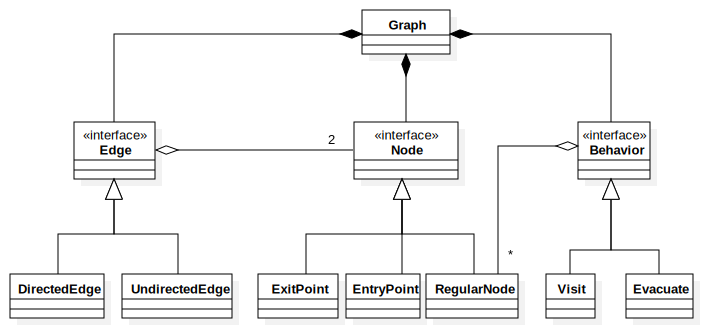
\includegraphics[width=\textwidth,height=\textheight,keepaspectratio]{images/graph-diagram.png}
\caption{Class diagram della struttura del grafo}
\label{fig:graph-diagram}
\end{figure}
Ogni behavior è caratterizzato da un identificatore, attribuitogli dal XML, e da una lista di nodi regolari di interesse che devono essere visitati prima di permettere all'attore di puntare ad una uscita. 

\subsection{Parser XML e Builder}
Come già accennato, abbiamo scelto il formato JDOM per la rappresentazione del file XML. La scelta di questo formato è stata dettata dalla sua struttura, che si adatta meglio ai nostri fini di sola lettura e non di manipolazione del documento.\\
\begin{figure}[htbp]
\centering
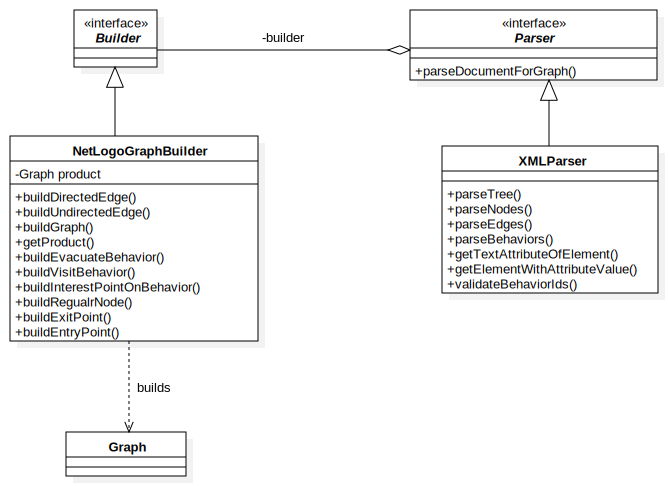
\includegraphics[width=\textwidth,height=\textheight,keepaspectratio]{images/builder-diagram.png}
\caption{Class diagram di Parser e Builder}
\label{fig:builder-diagram}
\end{figure}
Per la fase di costruzione delle classi abbiamo usato il pattern Builder, in modo da mantenere il processo di costruzione della struttura interna dell'oggetto di tipo Grafo trasparente all'utente di questo strumento. In particolare l'interfaccia del Builder aiuta a mantenere l'algoritmo di interpretazione dell'XML separato dal processo di costruzione e rappresentazione del suo contenuto in classi Java.\\
Il pattern Builder, inoltre, porta il grande beneficio di migliorare la modularizzazione derivante dall'incapsulamento di tutta la procedura di manipolazione della struttura interna dell'oggetto costruito, in questo modo il Client non ha necessità di conoscere la sua composizione interna.\\
Una conseguenza che rende il pattern ancora più adatto al nostro caso è il miglioramento del controllo sul processo di costruzione del prodotto. Al contrario di altri pattern creazionali, i quali costruiscono e restituiscono il prodotto in un'unica funzione, il Builder separa queste due operazioni mettendo a disposizione un'interfaccia più completa.\\
Grazie a questo noi siamo, quindi, in grado di esercitare un maggiore controllo sulla correttezza delle operazioni eseguite e delle informazioni inserite durante questa prima fase.\\
L'interfaccia Parser rende il progetto aperto ad estensioni future, come il supporto di linguaggi alternativi al XML.\\
\begin{figure}[htbp]
\centering
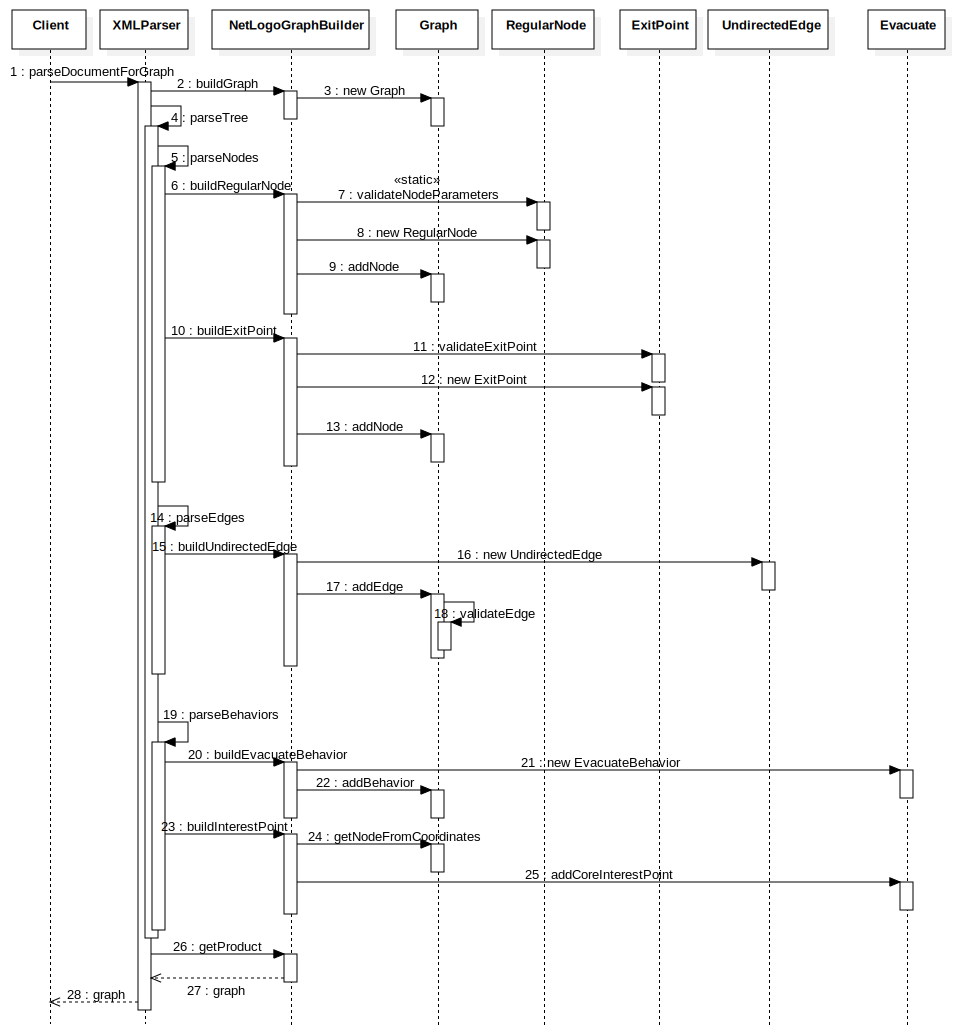
\includegraphics[width=\textwidth,height=\textheight,keepaspectratio]{images/builder-sequence.png}
\caption{Sequence diagram della costruzione di un grafo da parte di XMLParser}
\label{fig:builder-sequence}
\end{figure}
Come si vede in Figura \ref{fig:builder-diagram} il parser esercita il ruolo di Director per il builder. Il processo di analisi del documento e costruzione degli oggetti Java è descritto nel sequence diagram in Figura \ref{fig:builder-sequence}.
XMLParser costruisce, attraverso la libreria JDOM2, il modello JDOM del documento, il quale rispecchia la struttura ad albero del documento. Quindi il parser effettua una visita del modello ad albero, legge le informazioni necessarie e impartisce i corretti comandi al builder.\\

\subsection{Visitor}
Per l'operazione di scrittura del codice NetLogo si ha la necessità di estrapolare dagli oggetti che costituiscono la struttura del grafo diverse informazioni. Al variare della classe concreta varieranno anche le informazioni specifiche da estrarre.\\
Il grafo inoltre presenta una struttura di classi con interfacce diverse che devono, quindi, essere modificate per poter eseguire l'operazione necessaria.\\
In questo contesto, quindi, il pattern Visitor si rivela molto utile permettendo di eseguire operazioni specifiche al variare della classe concreta senza inquinare le diverse interfacce all'interno della struttura.\\
Un ulteriore vantaggio presentato dal Visitor è quello di concentrare le funzioni per la scrittura del codice NetLogo in classi specifiche rendendo il sistema più facile da manutenere ed eventualmente estendere.\\
La struttura dei modelli NetLogo finali è tale che gran parte del codice necessario rimane fissa al variare della simulazione, per questo motivo si ha che l'operazione di scrittura del codice NetLogo eseguita dai visitor è alternata a quella di lettura da appositi file di testo che contengono la parte fissa del modello. Queste parti fisse quindi vengono completate con le informazioni estrapolate dagli oggetti Java precedentemente messi in vita.\\
Abbiamo inoltre scelto di separare il modello NetLogo finale in due parti, mantenendo distinta la parte del modello che mette in vita l'ambiente da quella che controlla i movimenti degli attori e raccoglie le informazioni di interesse.\\
\begin{figure}[htb]
\centering
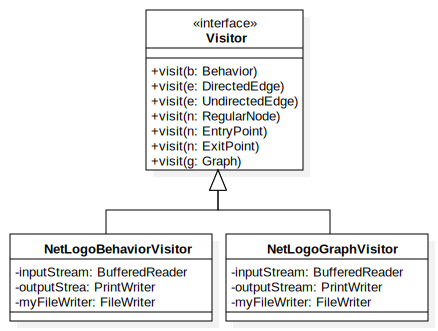
\includegraphics[width=\textwidth,height=\textheight,keepaspectratio]{images/visitor-class-diagram.png}
\caption{Class Diagram del Visitor}
\label{fig:visitor-diagram}
\end{figure}
Si hanno quindi due classi visitor distinte per ognuno dei due modelli NetLogo da creare: NetLogoGraphVisitor e NetLogoBehaviorVisitor ( Figura \ref{fig:visitor-diagram} ). Il primo effettua una visitita su nodi e archi del grafo per scrivere i comandi necessari a mettere in vita l'ambiente corretto. Il secondo, invece, effettua una visita sui behaviors in modo da definire i comportamenti che gli attori potranno avere nella simulazione e sui nodi per impostare lo stato iniziale del sistema.\\
In questo modo le interfacce delle classi del grafo, rimangono inalterate ma le operazioni effettuate variano al variare del visitor concreto, rendendolo un pattern ancora più adatto a questo specifico caso.\\
In Figura \ref{fig:visitor-sequence} è mostrato il funzionamento di un NetLogoGraphVisitor. L'oggetto finale ottenuto da questo visitor è un file eseguibile \texttt{.nlogo} che costruisce l'ambiente con la corretta topologia e esporta un file \texttt{.csv} necessario al secondo modello per l'acquisizione dell'ambiente.\\
\begin{figure}[htbp]
\centering
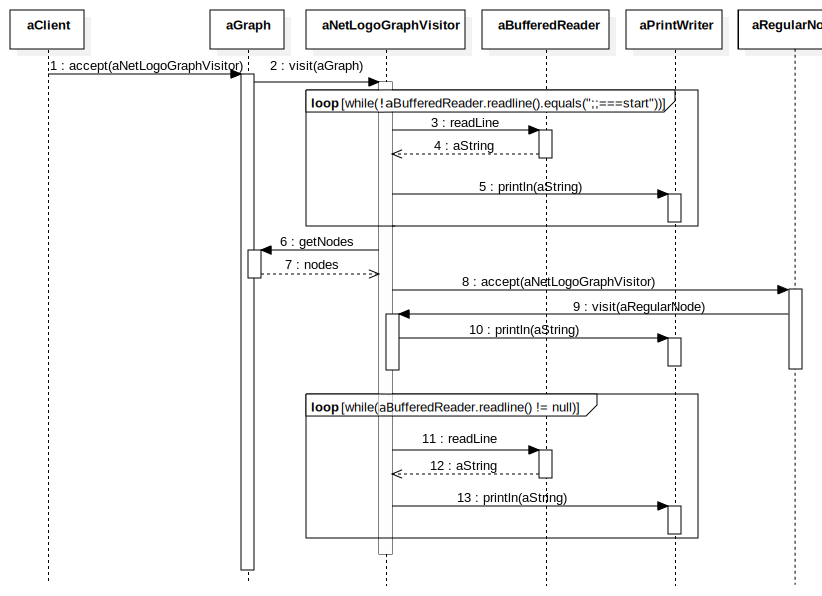
\includegraphics[width=\textwidth,height=\textheight,keepaspectratio]{images/visitor-sequence.png}
\caption{Sequence Diagram del NetLogoGraphVisitor su un grafo con un unico nodo}
\label{fig:visitor-sequence}
\end{figure}
NetLogoBehaviorVisitor, in modo analogo, eseguirà operazioni di lettura e scrittura alternate per generare un file eseguibile \texttt{.nlogo}.

\section{Modello NetLogo}
Come già accennato in precedenza abbiamo scelto di dividere il modello NetLogo generato dal nostro programma in due parti con lo scopo di mantenere le funzioni necessarie per la costruzione dell'ambiente separate da quelle che modellano i movimenti degli attori e raccolgono le informazioni sulla simulazione eseguita. In questo modo il codice è più facile da gestire e manutenere.\\
Questa scelta porta, inoltre, il vantaggio di poter sfruttare il file csv generato dal primo modello eseguendo questo una sola volta, in questo modo si evitano operazioni ridondanti nel caso in cui si vogliano simulare le interazioni di diversi comportamenti nello stesso ambiente.
\subsection{Ambiente}
L'ambiente in cui gli attori si muoveranno è modellato sotto forma di grafo con specifiche tipologie di turtles dette \texttt{beacon} che fanno da nodi e rappresentano quindi gli incroci tra le vie percorribili.\\
Gli archi sono rappresentati da due tipologie diverse di turtles dette \texttt{street}, percorribili in entrambi i versi, e \texttt{directed-street}, percorribili solo in un verso.\\
\begin{figure}[htbp]
\centering
\includegraphics[width=\textwidth,height=\textheight,keepaspectratio]{images/ambiente-screen.png}
\caption{Esempio di ambiente generato. In questo caso i beacons di ingresso sono di colore verde e i beacons di uscita di colore rosso.}
\label{fig:ambiente-screen}
\end{figure}
Per i beacons di ingresso e di uscita vengono anche impostati i relativi parametri, ovvero tasso di generazione o eliminazione degli attori e percentuali relative ai behavior da attribuire ad essi. In particolare per gli entry points si imposta anche un limite massimo del numero di attori che possono essere generati.\\
Grazie a questi parametri il sistema è predisposto per lo studio di simulazioni in ambienti comunicanti, in cui quindi gli attori possono uscire da un ambiente e entrare in un altro. 
\subsection{Behaviors e stato iniziale}
Abbiamo scelto di caratterizzare i behaviors degli attori con un identificatore intero e una lista di nodi di interesse che l'attore deve raggiungere prima di uscire dall'ambiente.\\
Sono state inoltre inserite due possibili modalità di raggiungimento dei beacons di interesse: ”\texttt{minDistance}” e “\texttt{orderedList}”. Nella prima l'attore punta al nodo più vicino a quello precedentemente raggiunto tra quelli di interesse, nella seconda invece la lista viene rigidamente percorsa rispettandone l'ordine.\\
Lo stato iniziale del sistema è contenuto in una semplice lista \texttt{initial-state} che viene percorsa da una apposita funzione per la corretta generazione degli attori sui vari nodi. 
\begin{figure}[htbp]
\centering
\includegraphics[width=\textwidth,height=\textheight,keepaspectratio]{images/movers-screen.png}
\caption{Esempio di ambiente popolato con attori nello stato iniziale. Gli attori hanno assunto il colore del beacon che hanno come obiettivo, in questo caso abbiamo un unico behavior che ha come interest point il beacon di colore rosa.}
\label{fig:movers-screen}
\end{figure}

\begin{figure}[htbp]
\centering
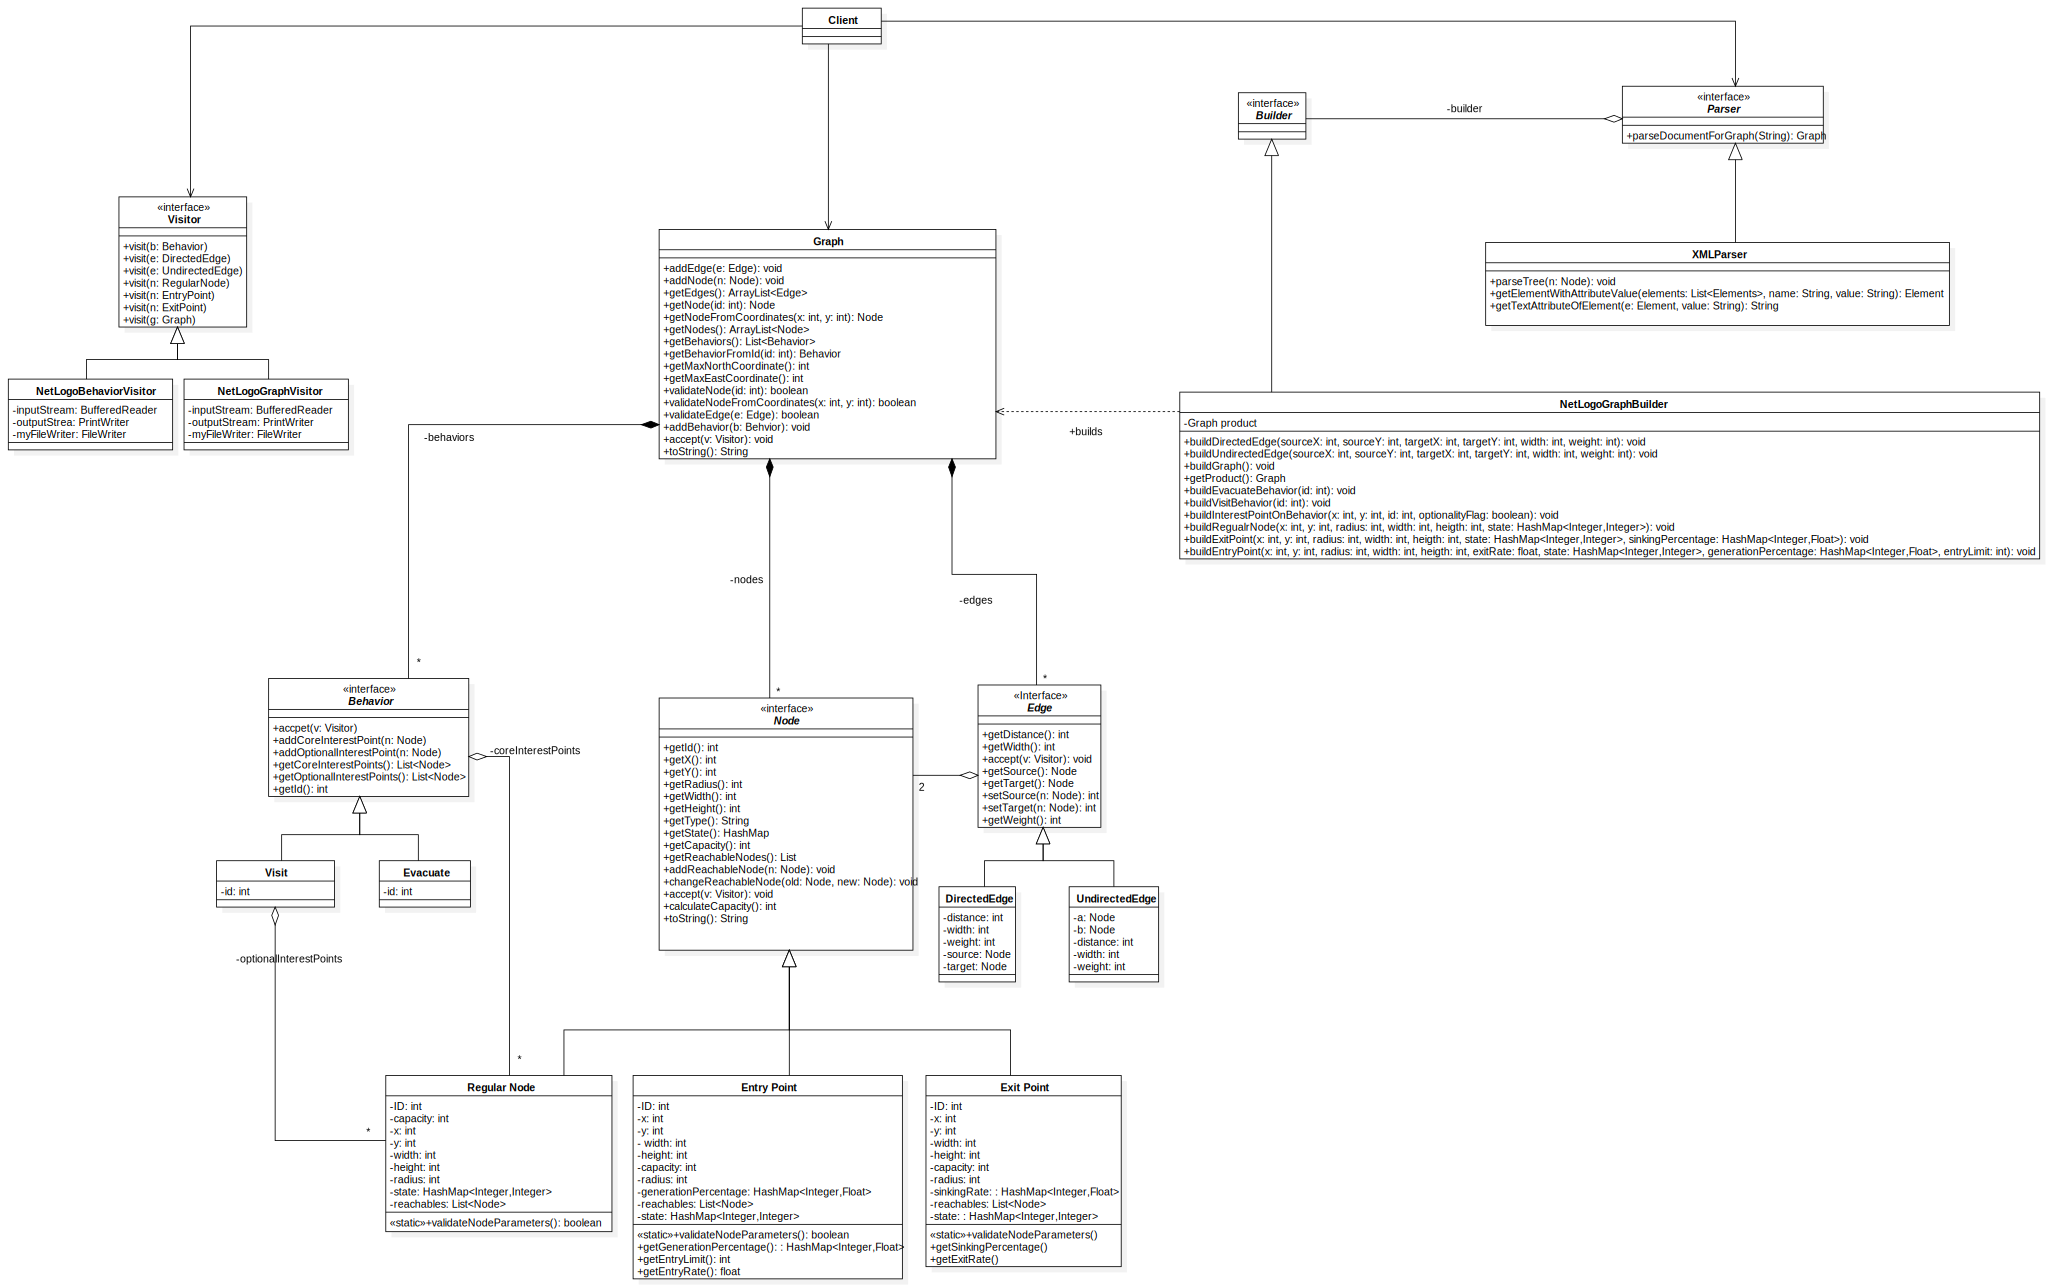
\includegraphics[width=\textwidth,height=\textheight,keepaspectratio]{images/complete-diagram.png}
\caption{Classi diagram}
\label{fig:complete-diagram}
\end{figure}